\documentclass[xcolor=dvipsnames]{beamer}
%\documentclass[handout,xcolor=dvipsnames,pdftex,hyperref={colorlinks=false}]{beamer}

% == Packages for beamer
\usepackage{xcolor}
\usepackage{graphicx}
\usepackage{fancybox}
\usepackage{hyperref}
\usepackage{amsmath,amssymb,amsfonts,bm}
\usepackage{wasysym}
\usepackage{colortbl}

\newcommand{\Plus}{\mathord{\tikz\draw[line width=0.3ex, x=1ex, y=1ex] (0.5,0) -- (0.5,1)(0,0.5) -- (1,0.5);}}

\usepackage{tikz}
\usetikzlibrary{positioning}
\usetikzlibrary{shapes,decorations,arrows,calc,arrows.meta} 
\tikzset{
	-latex,auto,node distance = 1.5cm and 1.5cm,
	semithick ,
	state/.style ={ellipse, draw, minimum width = 0.5 cm},
    old inner xsep/.estore in=\oldinnerxsep,
    old inner ysep/.estore in=\oldinnerysep,
	el/.style = {inner sep=2pt, align=left, sloped},
	point/.style = {circle, draw=black, inner sep=0.04cm,
	 fill=black,
                node contents={}},
}


\usepackage[english]{babel}
\usepackage{times}
\usepackage[T1]{fontenc}

% == Other Packages
\usepackage{rotating}
\usepackage{latexsym}
\usepackage{ulem}


% == theme & colors
\usetheme{Warsaw}  % Jens' previous
\usepackage{helvet}
\definecolor{someblue}{rgb}{0,.1,0.8}

% == New Commands
% = For general typesetting
\newcommand\spacingset[1]{\renewcommand{\baselinestretch}{#1}\small\normalsize}
\renewcommand\r{\right}
\renewcommand\l{\left}

\newcommand\makegaps{\addtolength{\itemsep}{.25\baselineskip}}
\newcommand\makebiggaps{\addtolength{\itemsep}{.5\baselineskip}}

% = For stats & econometrics
\renewcommand{\epsilon}{\varepsilon}
\newcommand\ud{\mathrm{d}}
\newcommand\dist{\buildrel\rm d\over\sim}
\newcommand\ind{\stackrel{\rm indep.}{\sim}}
\newcommand\iid{\stackrel{\rm i.i.d.}{\sim}}
\newcommand\logit{{\rm logit}}
\newcommand\cA{\mathcal{A}}
\newcommand\cN{\mathcal{N}}
\newcommand\E{\mathbb{E}}
\newcommand\V{\mathbb{V}}
\newcommand\cJ{\mathcal{J}}
\newcommand\y{{\bm y}}
\newcommand\Y{{\bm Y}}
\newcommand\X{{\bm X}}
\newcommand\x{{\bm x}}
\newcommand\eps{{\bm\varepsilon}}
\newcommand\zero{{\bm 0}}
\newcommand\be{{\bm\beta}}
\renewcommand\b{{\bm b}}
\newcommand\C{{\bm C}}
\newcommand\D{{\bm D}}
\newcommand\I{{\bm I}}
\newcommand\Z{{\bm Z}}
\newcommand\eeta{{\bm \eta}}
\DeclareMathOperator*\plim{plim}
\DeclareMathOperator\rank{rank}
\newcommand\indep{\protect\mathpalette{\protect\independenT}{\perp}}
\DeclareMathOperator{\sgn}{sgn}
\def\independenT#1#2{\mathrel{\rlap{$#1#2$}\mkern2mu{#1#2}}}

\newcommand{\notindep}{{\bot\negthickspace\negthickspace\bot}{\negthinspace
  \negmedspace \negthickspace \negthickspace \diagup
  \;}}

\newcommand{\bs}{\boldsymbol}
\newcommand{\mb}{\mathbf}
\newcommand{\real}{\mathbb{R}}
\renewcommand{\u}{\ensuremath{\mb{u}}}
\renewcommand{\v}{\ensuremath{\mb{v}}}
\newcommand{\U}{\ensuremath{\mb{U}}}
\newcommand{\M}{\ensuremath{\mb{M}}}
\renewcommand{\b}{\ensuremath{\bs{\beta}}}
\newcommand{\e}{\ensuremath{\bs{\epsilon}}}
\newcommand{\bhat}{\ensuremath{\hat{\bs{\beta}}}}
\newcommand{\XX}{\ensuremath{\X'\X}}
\newcommand{\XXinv}{\ensuremath{\left(\XX\right)^{-1}}}
\newcommand{\hatsig}{\ensuremath{\hat{\sigma}^2}}
\newcommand{\sig}{\ensuremath{\sigma^2}}
\newcommand{\hatmat}{\ensuremath{\X \XXinv \X'}}
\newcommand{\ehat}{\ensuremath{\hat{\e}}}
\newcommand{\tr}{\text{tr}}
\newcommand{\Sig}{\ensuremath{\bs{\Sigma}}}
\newcommand{\SigInv}{\ensuremath{\bs{\Sigma^{-1}}}}
\newcommand{\W}{\ensuremath{\mb{W}}}

\newtheorem{iass}{Identification Assumption}
\newtheorem{ires}{Identification Result}
\newtheorem{estm}{Estimand}
\newtheorem{esti}{Estimator}

\title[]{The Potential Outcome Framework, Part 1}
\subtitle[ ]{Stat 256, Causality}
\date{Spring 2026}
\author[Hazlett]{Chad Hazlett }
\institute[UCLA]{UCLA\\[1ex]
  \texttt{chazlett@ucla.edu}
}

\definecolor{dgreen}{rgb}{0,.6,0.8}
\newtheorem{assumption}{Assumption}
\useoutertheme{infolines}
\begin{document}

\subject{Talks}
\AtBeginSection[]
{
  \begin{frame}<beamer>
    \frametitle{Outline}
    \tableofcontents[currentsection]
  \end{frame}
}

\AtBeginSubsection[]
{
  \begin{frame}<beamer>
    \frametitle{Outline}
    \tableofcontents[currentsection,currentsubsection]
  \end{frame}
}

\begin{frame}
  \titlepage
\end{frame}

%\begin{frame}
%  \frametitle{Purpose, Scope, and Examples}
%Goal in causal inference is to assess the causal effect some potential cause (e.g. an institution, intervention, policy, or event) on some outcome.\\\bigskip
%
%Examples of such research questions include: What is the effect of
%\begin{itemize}
% \item political institutions on corruption?
% \item voting technology on  voting fraud?
% \item incumbency status on vote shares?
% \item peace-keeping missions on peace?
% \item mass media on voter preferences?
% \item church attendance on turnout?
%\end{itemize}
%\end{frame}

% Find somewhere to talk about where the POs are "primitives" or not.
% Say something about whether these are contradcitory approaches or not.

\begin{frame}{Readings}
Chapter 1-3 from Hernan \& Robins,  Causal Inference: What If. 
\end{frame}

\section{Potential Outcomes}

\begin{frame}
\frametitle{The Neyman-Rubin Potential Outcome Model}
\small
\onslide<1-> Much of the applied causal inference literature speaks the language of the \textcolor{Blue}{Neyman-Rubin causal model}, aka the \textcolor{Blue}{Potential Outcomes Model} (POM).\\
\bigskip

\begin{figure}
\begin{minipage}{.5\textwidth}
  \centering
  \includegraphics[width=.6\linewidth]{images/Neyman_3.jpeg}
  \caption{Neyman}
\end{minipage}%
\begin{minipage}{.5\textwidth}
  \centering
  \includegraphics[width=.5\linewidth]{images/DonRubin.jpg}
  \caption{Rubin}
\end{minipage}
\end{figure}
\end{frame}

\begin{frame}{What causal inference actually asks}
\onslide<1-> \textbf{What we do naturally:}
\begin{itemize}
\item Split units into a treated group and a control group
\item Compare average outcomes \textit{across groups}
\item ``College grads are more liberal than non-grads.''
\end{itemize}
\bigskip
\onslide<2-> \textbf{What causal inference asks:}
\begin{itemize}
\item For each unit, compare how they would do \textit{if treated} to how they would do \textit{if untreated}
\item ``Would \textit{this person} be more liberal \textit{if they got a degree} than \textit{if they didn't}?''
\end{itemize}
\bigskip
\onslide<3-> The first is a comparison \textit{between groups of different units}. The second is a comparison \textit{within each unit}, between two versions of its world.
\end{frame}

\begin{frame}{Group comparison vs. within-unit comparison}
\begin{center}
  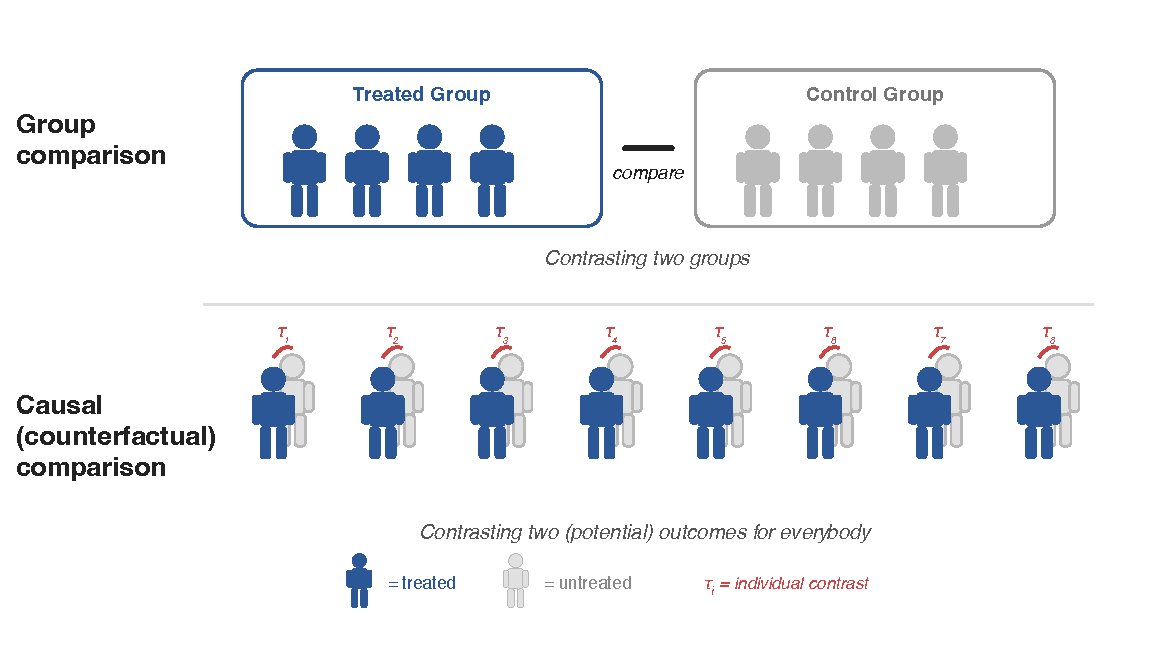
\includegraphics[width=\textwidth]{images/group_vs_counterfactual.pdf}
\end{center}
\end{frame}

\begin{frame}{Potential Outcomes, Labeled}
\vspace{-.05in}
\begin{center}
  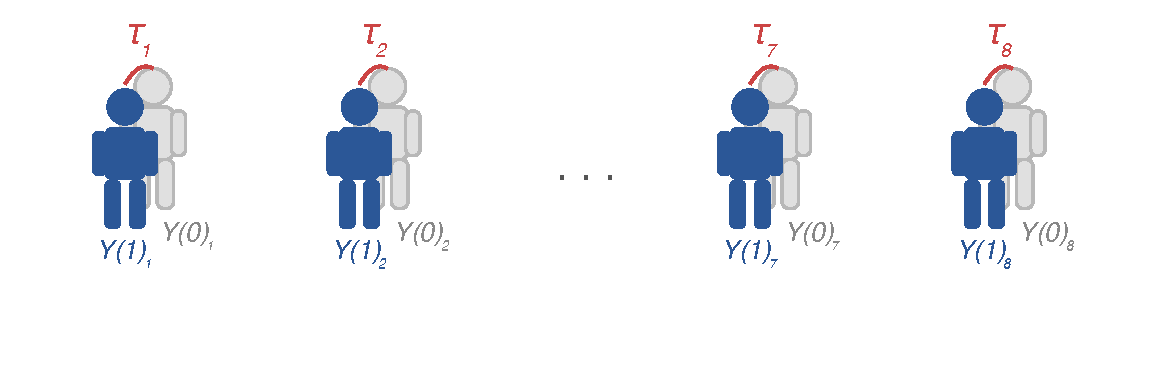
\includegraphics[width=\textwidth]{images/counterfactual_labeled.pdf}
\end{center}
\vspace{-.2in}
\small
\begin{itemize}
\item $\textcolor{Blue}{Y_{1i}}$: the outcome unit $i$ \textit{would have} under treatment
\item $\textcolor{Green}{Y_{0i}}$: the outcome unit $i$ \textit{would have} under control
\item $\textcolor{Red}{\tau_i} = Y_{1i} - Y_{0i}$: the causal effect for unit $i$
\end{itemize}
\textcolor{Red}{Fundamental problem}: we only ever see \textit{one} potential outcome per unit.
\end{frame}

\begin{frame}{From potential to observed}
\small
Adding the treatment indicator $D_i \in \{0,1\}$, the observed outcome is
\[
Y_i = D_i\,Y_{1i} + (1-D_i)\,Y_{0i}.
\]
\smallskip
Key idea: $D_i$ doesn't \emph{change} the potential outcomes --- it just picks which one you see.\\
\bigskip
\onslide<2-> Which of these are \textit{always}, \textit{sometimes}, or \textit{never} observable?
\begin{itemize}
\footnotesize
\item $D_i$ \quad\quad $Y_i$ \quad\quad $Y_{1i}$ \quad\quad $Y_{0i}$ \quad\quad $\tau_i$
\end{itemize}
\end{frame}

\begin{frame}{POs and QOIs}
\onslide<1->  Some quantities of interest will be:\\
\small
\begin{itemize}
\item<2-> Average treatment effect (ATE): $\E[Y_{1i}-Y_{0i}]=\E[\tau]$
\medskip
\item<3-> Average treatment effect on the treated (ATT)
\medskip
\[\E[\tau_i|D_i=1]=\E[Y_{1i}-Y_{0i}|D_i=1]\]
\item<4-> Average treatment effect on the controls (ATC)
\medskip
\[\E[\tau_i|D_i=0]=\E[Y_{1i}-Y_{0i}|D_i=0]\]

\item<5-> Conditional average treatment effect (CATE):
\medskip
\[\E[\tau_i|X=x]=\E[Y_{1i}-Y_{0i}|X=x]\]

\end{itemize}
\end{frame}

\begin{frame}{Visualizing the ATT}
\small
The ATT asks: among units actually treated ($D_i=1$), what's the average of their individual causal effects? Not a group comparison --- imagine each treated unit's two potential lives:
\begin{center}
  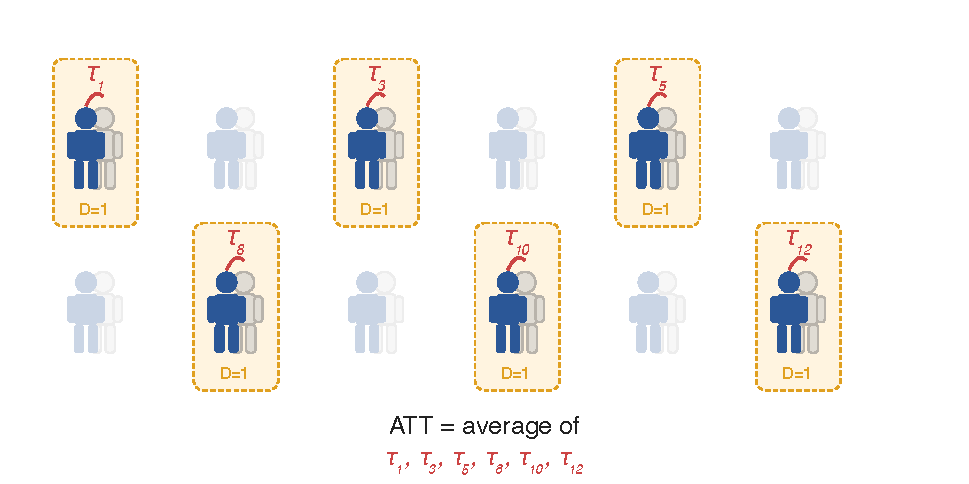
\includegraphics[width=0.85\textwidth]{images/att_visual.pdf}
\end{center}
\end{frame}

\begin{frame}{Visualizing the ATC}
\small
The ATC asks the same question for the untreated ($D_i=0$). These units were \textit{not} treated, but we still ask what \textit{would have happened} if they had been:
\begin{center}
  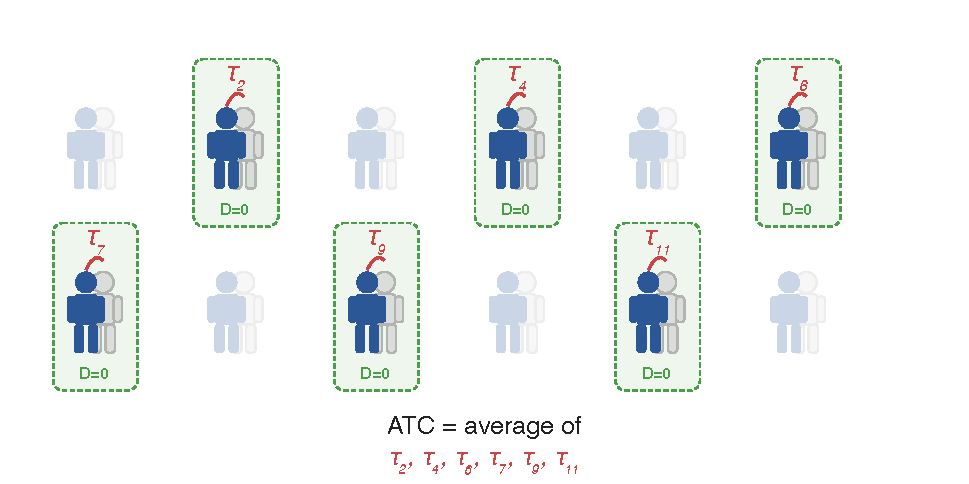
\includegraphics[width=0.85\textwidth]{images/atc_visual.pdf}
\end{center}
\end{frame}

\begin{frame}{The one embodied assumption: Consistency}
\small
\onslide<1-> By writing $Y_i(d)$ we assert \textbf{consistency}: $Y_i(d)$ is the $Y_i$ you'd see if $i$ actually received treatment $d$. We name it so we can reference it later and notice where it breaks.\\
\medskip
\onslide<2-> Main threat: \textbf{interference/spillovers}. If unit $j$'s treatment affects unit $i$'s outcome, then $Y_i(d)$ isn't well-defined without also specifying everyone else's status. (Think vaccines, education, monitoring.)\\
\medskip
\onslide<3-> You'll encounter \textbf{SUTVA} (Rubin 1980) = no interference + ``one version of treatment.'' Essentially this is just consistency when $d$ has a single well-defined value --- a re-statement, not a new assumption.\\
\medskip
\onslide<4-> \footnotesize (``One version of treatment'' is easy to overread; we'll save that for later.)
\end{frame}

\begin{frame}{Not every PO is a good PO}
\small
\onslide<1-> You can write $Y_i(d)$ for anything. That doesn't mean it's well-defined or that it's what you want.\\
\bigskip
\onslide<2-> \textbf{Requires clarification} --- what exactly are you changing?
\footnotesize
\begin{itemize}
\item Race, gender: when do you ``change'' it? In whose eyes?
\item Obesity: which feature of it?
\end{itemize}
\smallskip
\small
\onslide<3-> \textbf{Arguably ill-defined} --- the PO may not exist:
\footnotesize
\begin{itemize}
\item ``the size of the tumor in the brain of a patient who in fact died'' (truncation by death).
\end{itemize}
\smallskip
\small
\onslide<4-> A common guideline: a cause should be \textbf{manipulable} --- you should be able to describe an ideal experiment that would set $D=d$.
\footnotesize
\begin{itemize}
\item Helpful prodding, not a hard rule: non-manipulable things can have effects too, and the SCM can define those cleanly.
\end{itemize}
\end{frame}


%\begin{frame}{POs as primitives?}
%\small
%\onslide<1-> One bad habit is to take these potential outcomes as though they come out of nowhere. \\
%\bigskip
%\onslide<2-> This can make claims about how the POs relate to other quantities impossible to scrutinize. 
%\begin{itemize}
%\item<3-> e.g. how can you evaluate the assumption $\{ Y(1), Y(0)\}  \indep D | X$?
%\item<4-> (though you could do it via strong assumptions on $D|X$)
%\end{itemize}
%\bigskip
%\onslide<4-> But we need not be so primitive: yes the POs are RVs we write down, but they come from somewhere. Our SCM/graph already tells us where:
%\footnotesize
%\begin{itemize}
%\item unit potential outcomes:  $Y_{xi} = Y(do(X=x), U=u_i)$ 
%\item with distribution given by $P(Y_x) = P(Y|do(X=x))$ 
%\end{itemize}
%\end{frame}


\begin{frame}{Brain Training}
\textbf{Test 1}: Is $\E[Y_{1i}|D_i=1]=\E[Y_i|D_i=1]$?\\

\bigskip
\onslide<2-> What licenses this?

\end{frame}

\begin{frame}{Brain Training}
\onslide<1-> \textbf{Test 2}: Suppose $D_i$ randomly assigned. 
\small
\begin{itemize}
\item<2-> How would the $Y_{1i}$ you observed (i.e. when $D_i=1$) compare to the $Y_{1i}$ you don't observe? And for $Y_{0i}$?
\bigskip
\item<3-> What can we say about $\E[Y_{1i}|D_i=1]$ compared to $\E[Y_{1i}|D_i=0]$ and $\E[Y_{1i}]$?
\bigskip
\item<4->[] (While we're here: this is ignorability, aka exchangeability!)
\bigskip
\item<5-> So can we estimate $\E[Y_{1i}]$? And $\E[Y_{0i}]$?  How? What licenses do you use?
%\bigskip
%\item<6-> What does a sample estimator of $\E[Y_i|D_i=1]-\E[Y_i|D_i=0]$ tell us?
\end{itemize}
\end{frame}


\begin{frame}{Brain Training}
%\onslide<1-> \textcolor{Blue}{Recall $D_i$ is a ``switch'' that determines whether you see $Y_{1i}$ or $Y_{0i}$} \\
%\bigskip 
\onslide<1-> \textbf{Test 3}: Suppose $Y_{1i}=Y_{0i}$ for all $i$. But now, someone magically sees $Y_{1i}$, and chooses $D_i=1$ more often when $Y_{1i}$ is higher.
\small
\begin{itemize}
\item<2-> How would the $Y_{1i}$ you see compare to $Y_{1i}$ you don't see? 
\smallskip
\item<3-> So does $\E[Y_{1i}|D_i=1]=\E[Y_{1i}|D_i=0]=\E[Y_{1i}]$? 
\smallskip
\item<4-> How would the $Y_{0i}$ you see compare to the ones you don't?
\item<5-> If you estimate $\E[Y_i|D_i=1]-\E[Y_i|D_i=0]$, do you expect something near zero, positive, or negative? 
\item<6-> Does this tell us anything about $\E[Y_{1i}-Y_{0i}]$?
\item<7-> Can you say anything about expected direction of bias?
\end{itemize}
\end{frame}

\begin{frame}{Brain Training}
\onslide<1-> \textbf{Test 4}: Suppose you don't know anything about how $D_i$ is assigned w.r.t. $Y_{1i}$ and $Y_{0i}$. 
\bigskip
\begin{itemize}
\item<2-> Can we say anything about how $\E[Y_i|D_i=1]-\E[Y_i|D_i=0]$ compares to $\E[Y_{1i}]-\E[Y_{0i}]$?
\bigskip
\item<3-> Unfortunately, this is often the scenario we are in with observational data. 
\end{itemize}
\end{frame}

\begin{frame}{Brain Training: Visual Practice}
\small
\onslide<1-> Let's look at $Y_{1i}$ and $Y_{0i}$ alone first.\\
\vspace{-.4in}
\begin{center}
  \includegraphics[scale=.7]{y0y1plot_blank.pdf}
\end{center}
\vspace{-.2in}
\onslide<1-> True $\E[Y_{1i}-Y_{0i}]=\text{ATE}=3$\\
%\medskip
%\onslide<1-> %$\overline{Y}_{1i}-\overline{Y}_{0i}=\hat{ATE}=3.01$\\
\end{frame}

\begin{frame}{Random Assignment of Treatment}
\small
\onslide<1-> Now suppose $D_i=1$ is randomly assigned. We see only the filled dots:\\
\vspace{-.4in}
\begin{center}
  \includegraphics[scale=0.7]{y0y1plot_nobias.pdf}\\
\end{center}
\vspace{-.2in}
\onslide<2-> We get \[\hat{\E}[Y_i|D_i=1]-\hat{\E}[Y_i|D_i=0]=\widehat{\text{DIM}}=3.01 \;\approx\; \text{ATE}\]
\end{frame}

\begin{frame}{Selection into treatment, case 1}
\small
\onslide<1-> Suppose $Pr(D_i=1)$ increases to the right. Now we observe (filled dots):\\
\vspace{-.4in}
\begin{center}
  \includegraphics[scale=0.7]{y0y1plot_posbias.pdf}\\
\end{center}
\vspace{-.2in}
\onslide<2-> What difference in means do you expect?\\
\vspace{-.1in}
\onslide<3-> \[\hat{\E}[Y_i|D_i=1]-\hat{\E}[Y_i|D_i=0]=\widehat{\text{DIM}}=9.97 \;\neq\; \text{ATE}=3\]
\end{frame}

\begin{frame}{Selection into treatment, case 2}
\small
\onslide<1-> Now suppose $Pr(D_i=1)$ decreases to the right. We observe (filled dots):\\
\vspace{-.5in}
\begin{center}
  \includegraphics[scale=0.7]{y0y1plot_negbias.pdf}\\
\end{center}
\vspace{-.3in}
\onslide<2-> What difference in means do you expect now?
\vspace{-.05in} \onslide<3-> \[\hat{\E}[Y_i|D_i=1]-\hat{\E}[Y_i|D_i=0]=\widehat{\text{DIM}}=-1.59 \;\neq\; \text{ATE}=3\] \\
%\onslide<4-> Preview: Can't do anything about this yet, but if we observed ``$X$'',  some hope.
\end{frame}

%\begin{frame}{Preview of Things to Come}
%\footnotesize
%\onslide<1-> Again, say $Pr(D_i=1)$ decreases to the right\\
%\smallskip
%\onslide<2-> But now suppose $X$ is an observable, and $D$ is random conditional on $X$\\
%\vspace{-.5in}
%\begin{center}
%  \includegraphics[scale=0.6]{y0y1plot_negbias_X.pdf}\\
%\end{center}
%%\vspace{-.2in}
%%\[[\overline{Y}_i|D=1]-[\overline{Y}_{i}|D=0]=\widehat{ATE}=2.63\]
%\end{frame}
%
%\begin{frame}{Preview of Things to Come}
%\footnotesize
%\onslide<1-> Again, say $Pr(D_i=1)$ decreases to the right\\
%\smallskip
%\onslide<1-> But now suppose $X$ is an observable, and $D$ is random conditional on $X$\\
%\vspace{-.4in}
%\begin{center}
%  \includegraphics[scale=0.6]{y0y1plot_matched.pdf}\\
%\end{center}
%\vspace{-.2in}
%\onslide<1-> Having observed $X$ what if we compare treated to control only at starred points?  \\
%\onslide<2->
%\[[\overline{Y}_i|D=1]-[\overline{Y}_{i}|D=0]=\widehat{ATE}=2.63\]
%\end{frame}

%\begin{frame}{Notation and Definitions}
%\small \onslide<1-> Unit-level effects ($\tau_i$) are fundamentally unidentifiable.  On occasion we will be able to identify various average effects. Some estimands include: \\
%\footnotesize
%\begin{itemize}
%\item Treatment effect, $\tau_i = Y_{1i}-Y_{0i}$
%\item Average Treatment Effect (ATE):  
%\[ATE = \E[Y_{1i}-Y_{0i}] = \E[\tau_i] = \int \tau p(\tau) d\tau \]
%\item Average treatment effect on the treated (ATT):
%\[ATT = \E[Y_{1i}-Y_{0i}|D_i=1] = \int \tau p(\tau|D=1) d\tau\]
%\item Average treatment effect on the controls (ATC):
%\[ATC = \E[Y_{1i}-Y_{0i}|D_i=0] = \int \tau p(\tau|D=0) d\tau\]
%\item Average treatment effect for sub-groups ($ATE(X)$):
%\[ATE(X) = \E[Y_{1i}-Y_{0i}|X=x] = \int \tau p(\tau|X=x) d\tau \]
%\end{itemize}
%\end{frame}
%
%\begin{frame}{Practice}
%\small Looking at this plot, describe the meaning of the $ATE$, $ATT$, $ATC$, \& $ATE(X)$ graphically
%\begin{center}
% % \includegraphics[scale=.7]{y0y1plot_blank.pdf} 
%  \includegraphics[scale=0.6]{y0y1plot_negbias_X.pdf}\\
%\end{center}
%\end{frame}
%
%\begin{frame}[fragile]
%\frametitle{A Common Assumption: SUTVA}
%\small
%\onslide<1-> The use of notation $\{Y_{1i},Y_{0i}\}$  implicitly means we only care about treatment status of $i$ and not of other units, $j$ \\
%\footnotesize
%\begin{itemize}
%%\item We also defined ``observed'' wrt only to unit $i$'s treatment: $Y_i=Y_{1i} D_i +Y_{0i}(1-D_i)$ 
%\item And we defined the causal effect $\tau_i$ as $Y_{1i}-Y_{0i}$
%\end{itemize}
%\small
%\medskip
%\onslide<2-> Known as Stable Unit Treatment Value Assumption (SUTVA), ``no interference'', or ``individualized treatment response''. \\ 
%\medskip
%\onslide<3-> It is easy to break: disease, vaccination, conflict, education, anti-corruption monitoring, ... \\
%\medskip
%\onslide<4-> Without this you get a proliferation of potential outcomes. E.g. with four units you could define:\\
%\[\{Y_i(0,0,0,0), Y_i(0,0,0,1),..., Y_i(1,1,1,1)\}\]
%\vspace{-.2in}
%\begin{itemize}
%\item<5-> how many potential outcomes for each unit, $i$? \\
%\item<6-> and how many causal effects for $i$?
%\end{itemize}
%\end{frame}
%
%\begin{frame}{Potential Outcomes with Interference}
%\small
%\begin{definition}[SUTVA]
%Unit $i$'s potential outcomes depend on $D_i$ and not on $D_{j \neq i}$
%\end{definition}
%\begin{itemize}
%\item<2-> e.g. $Y_3(0,0,D_3,0)$ is same as $Y_3(0,1,D_3,1)$, $Y_3(1,1,D_3,0)$,... 
%\item<3-> So just write $Y_3(D_3)$
%\item<4-> Also limits the causal effects for each unit: simply $\tau_i=Y_i(1)-Y_i(0)=Y_{1i}-Y_{0i}$
%\end{itemize}
%\bigskip
%\onslide<5-> This is an example of an \textbf{exclusion restriction}: we use outside information to rule out possibility of certain
%causal effects.
%\begin{itemize}
%\item<6-> the effect of you taking the treatment on my POs is excluded (0)
%\item<6-> traditional models (e.g. regression) do same: $Y_i$ depends on $X_i$ not $X_j$.
%\end{itemize}
%\onslide<7-> Causal inference in the presence of interference is an
%area of active research. e.g. sometimes ``spillover'' or ``saturation'' is deliberately varied 
%\end{frame}

\begin{frame}{Yet More Brain Training: ``science'' tables}
Imagine a study population with 4 units:

\begin{table}[ht]
    \centering
    \begin{tabular}{c  c c c c }
      $i$ & $D_i$ & $Y_{1i}$ & $Y_{0i}$ & $\tau_i$ \\ \hline
      1  & 1 & 10  & 4 & 6 \\
      2  & 1 & 1  & 2 & -1 \\
      3 & 0 & 3 & 3 & 0 \\
      4 & 0 & 5 & 2 & 3 \\
    \end{tabular}
    \end{table}

\onslide<2-> 1. What is the ATE?
\onslide<3-> \small $\E[Y_{1i} - Y_{0i}] = 1/4 \times (6-1+0+3)=2$ \\
\medskip
\footnotesize(Note: average effect is positive, but not all $\tau_i$ are)\\
\small
\medskip
\onslide<4-> 2. What are the ATT and ATC? \\
\begin{itemize}
\item<5->[] $\E[Y_{1i}-Y_{0i}|D_i=1]=.5(6-1)=2.5$\\
\item<6->[] $\E[Y_{1i}-Y_{0i}|D_i=0] =.5(0+3)=1.5$
\end{itemize}
\end{frame}

\begin{frame}{Difference in Means}
\small
\onslide<1-> You saw earlier how simple comparison of observed outcomes can be misleading. Let's use POM to see this more rigorously. \\
\bigskip
\onslide<2-> The \textcolor{Blue}{Difference in Means} estimand:
 $$\E[Y_i|D_i=1]-\E[Y_i|D_i=0]$$ \\
\bigskip
\onslide<3-> What does the POM tell us about this quantity? One decomposition:

\footnotesize
\begin{align*}
\E[Y_i|D_i=1]-\E[Y_i|D_i=0] &= \E[Y_{1i}|D_i=1]-\E[Y_{0i}|D_i=0] \\
%&= \textcolor{Blue}{\E[Y_{1i}|D_i=1]-\E[Y_{0i}|D_i=1]} + \textcolor{Green}{\left(\E[Y_{i0}|D_i=1]-\E[Y_{0i}|D_i=0] \right)} \\
&= \textcolor{Blue}{\E[Y_{1i}-Y_{0i}|D_i=1]} + \textcolor{Green}{\left(\E[Y_{0i}|D_i=1]-\E[Y_{0i}|D_i=0] \right)}
\end{align*}
\small
\onslide<4-> What are the terms in \textcolor{Blue}{blue} \& \textcolor{Green}{green}?

%\begin{scriptsize}
%\begin{align}
%\begin{split}
%E[Y_i|D=1]-E[Y_i|D_i=0] \\
%&=E[Y_{1i} | D_i=1]-E[Y_{0i} | D_i=0]\\
%                 &=\underbrace{E[Y_{1i} - Y_{0i} | D_i=1]}_{\mbox{ATT}}
%                 +\underbrace{\{ E[Y_{i0} | D_i=1]- E[Y_{0i} | D_i=0]\}}_{\mbox{BIAS}}\nonumber
%\end{split}
%\end{align}
%\end{scriptsize}
%
%\begin{itemize}
%\itemsep1pt\parskip0pt\parsep0pt
%\item
%  Bias term unlikely to be 0 in most applications.
%\item
%  Selection into treatment is often associated with the potential
%  outcomes
%\end{itemize}
\end{frame}

%\begin{frame}{Selection Bias}
%\footnotesize
%\begin{align*}
%\E[Y_i|D_i=1]-\E[Y_i|D_i=0] &= \E[Y_{1i}|D_i=1]-\E[Y_{0i}|D_i=0] \\
%&= \textcolor{Blue}{\E[Y_{1i}-Y_{0i}|D_i=1]} + \textcolor{Green}{\left(\E[Y_{0i}|D_i=1]-\E[Y_{0i}|D_i=0] \right)}
%\end{align*}  \\
%\medskip
%\onslide<1-> Can you think of an example and what these two values might look like? \\
%\medskip
%%\onslide<2-> Example: $D=\text{Church Attendance}$, $Y=\text{Political Participation}$ \\
%%\begin{itemize}
%%\item Church goers likely to differ from non-Church goers on a range of background characteristics (e.g.~civic duty)
%%\medskip
%%\item Turnout for churchgoers could be higher than for non-churchgoers even if churchgoers never attended church, or church had zero mobilizing effect
%%  ($\E[Y_{0i}|D_i=1]-\E[Y_{0i}|D_i=0]>0$)
%%\end{itemize}
%%\bigskip
%\onslide<2-> Example: Human rights treaties
%\begin{itemize}
%\item Countries willing to sign a human rights treaty will often be those with better human rights already. 
%\medskip
%\item Human rights better in signatory countries even if they had not signed ($\E[Y_{0i}|D_i=1]-\E[Y_{0i}|D_i=0]>0$)
%\end{itemize}
%\end{frame}

\begin{frame}{Summing Up: The Potential Outcomes Model}
\footnotesize
\begin{itemize}
\item<1-> \textbf{Causality is a within-unit comparison.} $\tau_i = Y_i(1)-Y_i(0)$ --- not a contrast between a treated group and a control group, but between two versions of the same unit's world, then averaged.
\medskip
\item<2-> \textbf{The fundamental problem.} You only ever see one of $Y_i(1), Y_i(0)$. Every causal question is a missing-data problem.
\medskip
\item<3-> \textbf{One embodied assumption: consistency.} Writing $Y_i(d)$ already asserts it. Interference is the main way it breaks; SUTVA is just consistency when $d$ is well-defined.
\medskip
\item<4-> \textbf{POs are a language, not a free lunch.} You can write $Y_i(d)$ for anything, but some POs are ill-defined (truncation by death) or not what you actually want. The notation doesn't rescue a bad question.
\medskip
\item<5-> \textbf{Next:} what has to be true about how $D$ is assigned for the observed difference to recover a causal quantity? $\rightarrow$ randomization, selection-on-observables, and the rest of the course.
\end{itemize}
\end{frame}

\end{document}
